\documentclass{beamer}

\usepackage[T1]{fontenc}
\usepackage[utf8]{inputenc}
\usepackage[italian]{babel}
\usepackage{graphicx}
\usepackage{booktabs}
\usepackage{wrapfig}
\usepackage{xargs}
\usepackage{multicol}
\usepackage{minted}
\usepackage{csquotes}
%\usepackage[backend=biber,style=reading,sorting=none]{biblatex}

\mode<presentation> {
    \usetheme{Boadilla}
    \usecolortheme{beaver}
}

\title[Navigazione cognitiva in Alchemist]{
    Simulazione di evacuazione di folle in Alchemist: \\
    un modello di mappa mentale per pedoni cognitivi
}

\author{Lorenzo Paganelli}

\institute[]
{
    Alma Mater Studiorum $\cdot$ Università di Bologna\\
    Campus di Cesena%
}

\date{19 Marzo 2020}

\begin{document}

\begin{frame}
  \titlepage
\end{frame}

% Uncomment these lines for an automatically generated outline.
%\begin{frame}{Outline}
%  \tableofcontents
%\end{frame}

%\section{Disastri}
\definecolor{bostonuniversityred}{rgb}{0.8, 0.0, 0.0}

\begin{frame}{Eventi rilevanti}
\hfil\hfil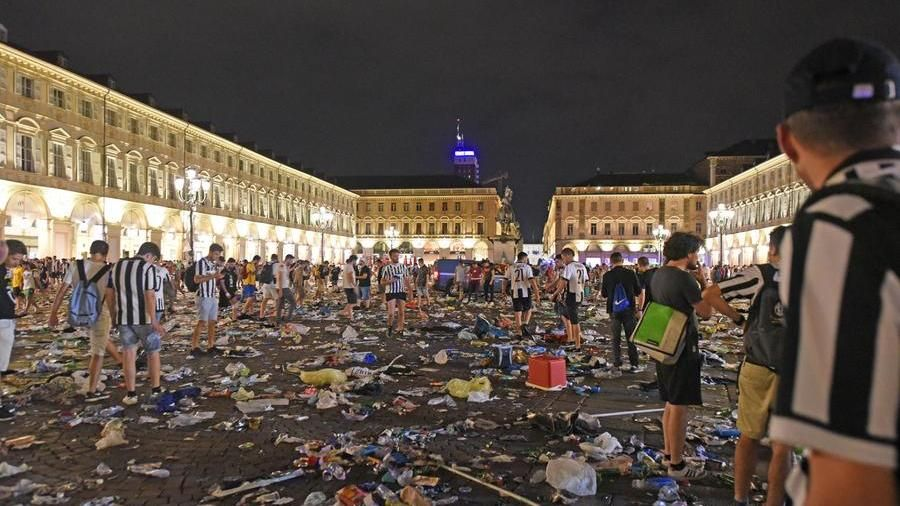
\includegraphics[width=5cm]{figures/piazza-san-carlo.jpeg}
\hfil\hfil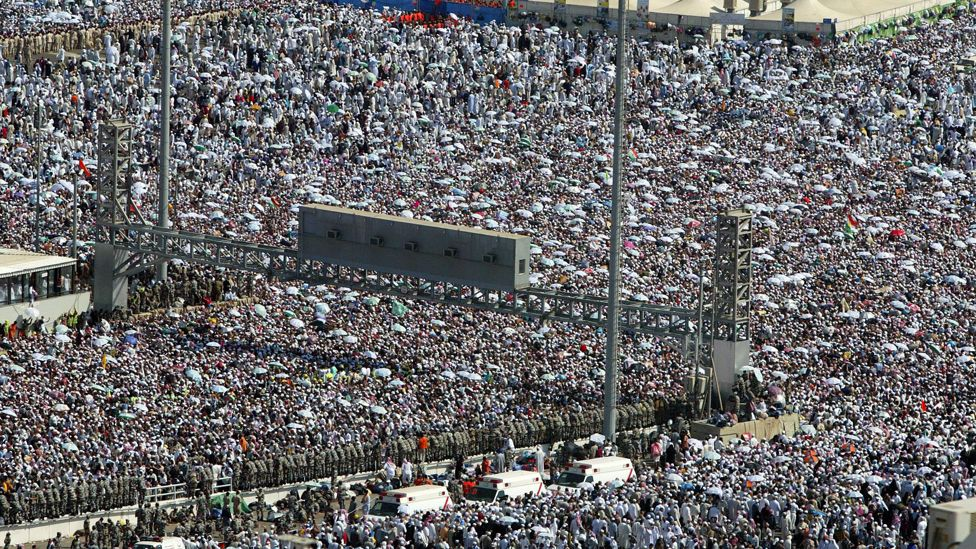
\includegraphics[width=5cm]{figures/hajj.jpg}
\newline
\null
\hfil\hfil\makebox[5cm]{Piazza San Carlo, Torino}
\hfil\hfil\makebox[5cm]{Ponte Jamarat, Mina}

\begin{block}{Conseguenze}
\begin{itemize}
    \item In Piazza San Carlo a Torino la fuga incontrollata della folla a seguito dell'uso di spray urticante da parte di malviventi causò 1500 feriti e 3 morti (2017)
    \item Sul Ponte Jamarat a Mina l'impatto tra due flussi di fedeli diretti verso la Mecca causò più di 2000 morti (2015)
\end{itemize}
\end{block}
\end{frame}

\begin{frame}{Simulazioni di evacuazione}
%\begin{block}{Soluzione}
%Per prevenire situazioni disastrose vengono solitamente effettuate delle simulazioni di evacuazione in vari scenari
%\end{block}
\begin{block}{Simulazioni reali}
\begin{itemize}
    \item Coinvolgono individui reali
    \item I costi possono essere proibitivi
    \item Le condizioni psicologiche dei partecipanti sono differenti rispetto a una situazione di vero o presunto pericolo
\end{itemize}
\end{block}
\begin{block}{Simulazioni computerizzate}
\begin{itemize}
    \item Coinvolgono individui simulati
    \item Sono in grado di valutare più scenari in minor tempo
    \item I costi sono più contenuti rispetto a simulazioni reali
    \item Sono inevitabilmente meno realistiche, ma possono essere utili per avere dei riscontri fin da subito
\end{itemize}
\end{block}
\end{frame}

\begin{frame}{Il simulatore Alchemist}
\begin{block}{Alchemist è}
\begin{itemize}
    \item Un simulatore nato all'interno dell'Università di Bologna che consente la simulazione di vari scenari, tra cui l'\textcolor{bostonuniversityred}{evacuazione di folle}
    \item Basato sul modello ad agenti: ciascun individuo è autonomo ed è rappresentato separatamente, dunque c'è eterogeneità
\end{itemize}
%\begin{itemize}
%    \item Un simulatore nato all'interno dell'Università di Bologna che consente la simulazione di vari scenari
%    \item Dotato delle astrazioni necessarie a simulare l'evacuazione di folle
%\end{itemize}
\end{block}
\begin{block}{In Alchemist sono modellati}
%\begin{block}{I pedoni simulati in Alchemist sono dotati di}
\begin{itemize}
    \item Aspetti fisici, come sesso ed età
    \item Aspetti psicologici, come paura e sensazione di pericolo
    \item Aspetti sociali, come la tendenza a rimanere vicino al proprio gruppo
    \item Interazioni psicologiche, come il contagio sociale
\end{itemize}
\end{block}
\begin{alertblock}{Problema}
I pedoni simulati in Alchemist sono sprovvisti della capacità di orientarsi
\end{alertblock}
\end{frame}

\begin{frame}{Pathfinding}
\begin{block}{Il pathfinding}
\begin{itemize}
    \item Consiste nell'individuazione del percorso più breve esistente tra due punti in un dato ambiente con ostacoli
    \item E' usato in alcuni modelli per risolvere il problema dell'orientamento dei pedoni simulati
    \item E' scomponibile in due sotto-problemi:
    \begin{enumerate}
        \item Ricavare dall'ambiente una struttura dati utile a trovare dei cammini minimi. Solitamente si usa un grafo i cui nodi sono \textcolor{bostonuniversityred}{poligoni convessi} che descrivono le aree dall'ambiente attraversabili dai pedoni (\emph{walkable areas}), mentre gli archi rappresentano le connessioni tra queste
        \item Trovare un cammino minimo tra due nodi di un grafo
    \end{enumerate}
\end{itemize}
\end{block}
\end{frame}

\begin{frame}{Human wayfinding}
\begin{alertblock}{Problema}
Il pathfinding assume che ogni pedone conosca perfettamente topologia e metriche dell'ambiente, ma questa ipotesi raramente è verificata: individui diversi hanno una \textcolor{bostonuniversityred}{conoscenza diversa} dello spazio circostante, spesso parziale e inaccurata
\end{alertblock}
\begin{block}{Soluzione}
\begin{itemize}
    \item Modellare l'inaccurata rappresentazione mentale che ciascun pedone ha dell’ambiente circostante, nota come mappa cognitiva
    \item Modellare il processo mentale che usa tali informazioni per orientarsi
\end{itemize}
\end{block}
\begin{block}{Più in generale}
Si vuole simulare la capacità umana di navigare l'ambiente, questo problema è noto come \textcolor{bostonuniversityred}{human wayfinding}
\end{block}
\end{frame}

\begin{frame}{Conoscenza spaziale 1/2}
\begin{block}{La mappa cognitiva è}
\begin{itemize}
    \item La rappresentazione mentale di un individuo dell’ambiente circostante
    \item Composta da \textcolor{bostonuniversityred}{landmark} (elementi dell'ambiente memorizzati per la loro unicità, ad esempio una torre) e relazioni spaziali tra questi %\cite{Andresen2018}
    \item Incompleta e inaccurata
    %\item La principale fonte di informazioni spaziali
\end{itemize}{}
\end{block}{}
\begin{block}{La si può modellare}
\begin{itemize}
    %\item Mediante un grafo i cui nodi sono landmark
    \item Rappresentando i landmark con delle \textcolor{bostonuniversityred}{ellissi}, in grado di descrivere l'imprecisione riguardo l'esatta posizione del landmark
    \item Memorizzando un'informazione booleana per ogni connessione tra landmark (non viene memorizzato il percorso)
\end{itemize}
\end{block}
\begin{block}{In generale}
Il grado di familiarità di un individuo con l'ambiente dipende dal numero di landmark e di connessioni nella sua mappa cognitiva
\end{block}{}
\end{frame}{}

\begin{frame}{Conoscenza spaziale 2/2}
\begin{alertblock}{Problema}
Che fare delle informazioni apprese dai pedoni durante la simulazione?
\end{alertblock}
\begin{block}{Soluzione}
\begin{itemize}
    \item Idealmente, si vorrebbe che tali informazioni si aggiungessero alla mappa cognitiva
    \item Per semplicità, si modella solo la capacità di ricordare e riconoscere aree dell'ambiente già visitate durante l'evacuazione
\end{itemize}
\end{block}
\begin{block}{La memoria volatile}
\begin{itemize}
    \item Consta delle informazioni spaziali che il pedone apprende durante l’evacuazione
    \item E' modellata con una mappa che ad ogni walkable area associa il numero di visite
\end{itemize}{}
\end{block}{}
\end{frame}

\begin{frame}{Elaborazione di informazioni spaziali 1/2}
\begin{alertblock}{Problema}
Dalla mappa cognitiva si può ricavare un percorso verso una destinazione marcata con un landmark speciale. Come si può seguire tale percorso?
\end{alertblock}{}
\hfil\hfil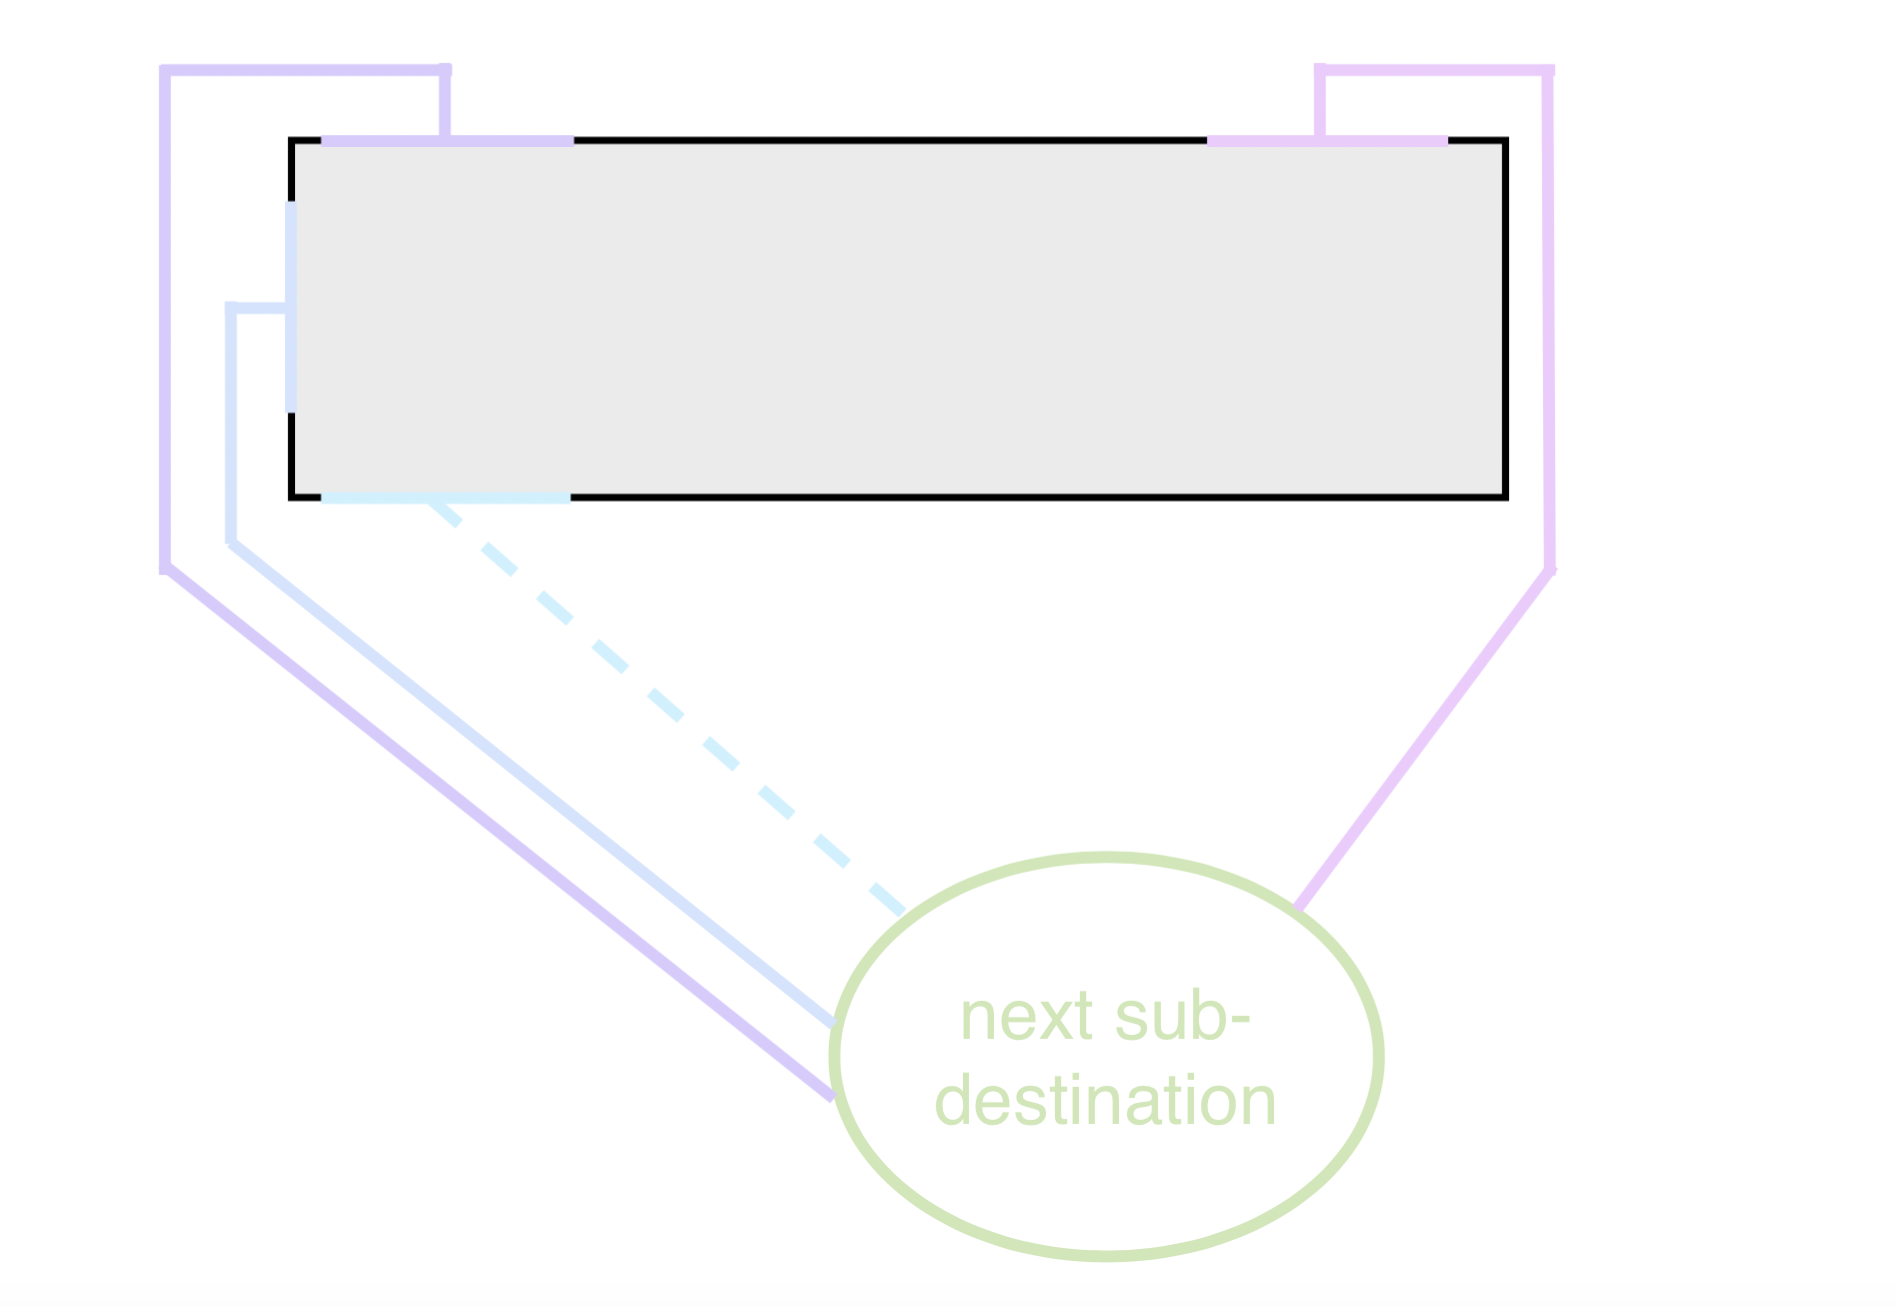
\includegraphics[width=9cm]{figures/polygonal-chains-to-subdestination.png}

\end{frame}{}

\begin{frame}{Elaborazione di informazioni spaziali 2/2}
\begin{block}{Il sistema di pesi}
Assegna un peso ad ogni arco incidente sulla walkable area in cui il pedone si trova, l'arco di peso minimo viene poi attraversato
\begin{equation}
    w(e) = f_{volatile\ memory}\cdot f_{cognitive\ map}\cdot f_{final}\cdot f_{impasse}\cdot f_{congestion}
\end{equation}{}
\begin{itemize}
    \item \(f_{volatile\ memory}\) aumenta il peso di archi conducenti a zone già visitate
    \item \(f_{cognitive\ map}\) riduce il peso di un arco in base a quanto questo permette di avvicinarsi al prossimo landmark
    \item \(f_{final}\) tiene conto di eventuali destinazioni trovate strada facendo
    \item \textcolor{bostonuniversityred}{\(f_{impasse}\)} aumenta il peso di archi conducenti a vicoli ciechi se presenti nella memoria volatile
    \item \textcolor{bostonuniversityred}{\(f_{congestion}\)} aumenta il peso di archi conducenti a zone affollate
\end{itemize}
\end{block}
\end{frame}

\begin{frame}{Esempi di simulazione}
\begin{block}{Conoscenza completa}
Un pedone con conoscenza completa dell'ambiente deve raggiungere una destinazione marcata di verde
\end{block}
\begin{block}{Conoscenza parziale (30\%)}
Un pedone con conoscenza parziale dell'ambiente (30\%) deve raggiungere una destinazione marcata di verde
\end{block}
\begin{block}{Nessuna conoscenza}
Un pedone senza conoscenza dell'ambiente deve raggiungere una destinazione marcata di verde
\end{block}
\begin{block}{Aggiramento delle congestioni}
130 pedoni devono raggiungere una destinazione in verde, ma i due percorsi più brevi sono affollati da persone senza capacità locomotorie
\end{block}
\end{frame}{}

\begin{frame}{Riferimenti}
    \nocite{*}
    \bibliographystyle{plain}
    \bibliography{bibliography}
\end{frame}

\end{document}
